\documentclass{article}
\usepackage{amsmath}
\usepackage{float}
\usepackage{graphicx}
\title{CSCE 452 Project 4 Report}

\author{Raegan Lucero
\and
 Caleb McWilliams
\and
 Daniel Bartel}
\date{}

\begin{document}
\maketitle

\section*{Wheel and Sensor Definitions}

The Vehicle has two wheels W1 and W2 and two sensors S1 and S2. The vehicle is shown below:
\begin{center}
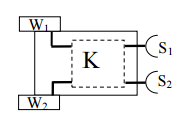
\includegraphics{vehicle}
\end{center}
The Relationship between wheel movement speed and sensor inputs are:
\begin{center}
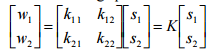
\includegraphics{Wheelspeeds}
\end{center}
It should be noted for K that a direct connection is:
\begin{center}
$
\begin{bmatrix}
1 & 0\\

0 & 1 \\

\end{bmatrix}
$
\end{center}
It is inputted by typing in 1001 when inserting the vehicle.

An crossed connection is:
\begin{center}
$
\begin{bmatrix}
0 & 1\\

1 & 0 \\

\end{bmatrix}
$
\end{center}
\section*{Speed Calculation}
For each movement a function called move is called. This function first calls calculateSpeed for each vehicle. The first thing that the calculateSpeed function does is calculate the distance for each light between the light and each wheel. To get S1 and S2 we simply divide 100 by the distance between the respective sensor. Next we solve for w1 and w2 by using k and s like so:

\begin{center}
w1 = k11 * S1 + K12 * S2 \\
w2 = K21 * S1 + K22 *  S2
\end{center}

This means that wheel one should move W1 pixels and Wheel two should move W2 pixels. Thus W1 and W2 are vectors in the direction that the vehicle is facing.

\section*{Direction Calculation}

The move function checks which direction the vehicle is tiled. It does this by checking the Y values of the wheel positions. Next it calculates the angle that the vehicle forms with the x plane. \\
If it is titled left:\\

Difference = Distance between the higher wheel and the lower wheel in the x direction / Distance between the wheels \\
angle = 180 - 90 - acos(Difference)\\


If it is titled right:\\

Difference = Distance between the higher wheel and the lower wheel in the x direction / Distance between the wheels\\
angle = acos(Difference) - 90\\

Then the new x and y positions of the wheels are defined as follows
\begin{center}
x(new) = x(old) - cos(angle)*speed of the wheel\\
y(new) = y(old) - sin(angle)*speed of the wheel\\
\end{center}

Note: speed of wheel is w1 and w2\\
    subtraction is used because of the orientation of the x y plane in the language\\
    
We then repeat the process of finding the tilt as above and calculate the new angle formed with the change of the wheel positions\\

Next we calculate the position of the upper points with the following formula

\begin{center}
x(new) = x(old) - cos(angle)*75\\
y(new) = y(old) - sin(angle)*75\\
\end{center}

Note: 75 is the distance between the front and back of the vehicle (the length)\\
    
Lastly we call redraw() which updates the position of the vehicle on the screen. It should be noted that when the movement is toggled on the move function is called repeatedly. 
\end{document}
